%%----------------------------------------------------------------------------------------
%	PACKAGES AND THEMES
%----------------------------------------------------------------------------------------
\PassOptionsToPackage{table}{xcolor}
\documentclass[aspectratio=169,xcolor=dvipsnames,svgnames,x11names,fleqn]{beamer}
% \documentclass[aspectratio=169,xcolor=dvipsnames,fleqn]{beamer}

\usetheme{RedVelvet}

\usefonttheme[onlymath]{serif}
\newcommand{\showanswers}{yes}


\usepackage{xspace}
\usepackage{amsmath}
\usepackage{amssymb}
\usepackage{amsfonts}
\usepackage{color}
\usepackage{physics}
% \usepackage{mathbb}
\usepackage{rahul_math}
\usepackage{bigints}

\usepackage{graphicx} % Allows including images
\usepackage{booktabs} % Allows the use of \toprule, \midrule and \bottomrule in tables
\usepackage{tikz,pgfplots}

\usepackage{subfigure}
\usetikzlibrary{arrows}
\usepackage{minted}
\definecolor{LightGray}{gray}{0.9}
\definecolor{cream}{rgb}{0.92, 0.9, 0.55}
\definecolor{lightblue}{rgb}{0.68, 0.85, 0.9}


\usepackage{xcolor-material}
\usetikzlibrary{fit}
\usetikzlibrary{matrix}
\tikzset{%
apple/.pic={
    \fill [MaterialBrown] (-1/8,0)  arc (180:120:1 and 3/2) coordinate [pos=3/5] (@)-- ++(1/6,-1/7)  arc (120:180:5/4 and 3/2) -- cycle;
    \fill [MaterialLightGreen500] (0,-9/10)  .. controls ++(180:1/8) and ++(  0:1/4) .. (-1/3,  -1) .. controls ++(180:1/3) and ++(270:1/2) .. (  -1,   0) .. controls ++( 90:1/3) and ++(180:1/3) .. (-1/2, 3/4) .. controls ++(  0:1/8) and ++(135:1/8) .. (   0, 4/7)
    }
    }

\newcommand{\leftdoublequote}{\textcolor{blue}{\scalebox{3}{``}}}

\newcommand{\rightdoublequote}{\textcolor{blue}{\scalebox{3}{''}}}


\usepackage{textcomp}
\usepackage{fontawesome}
\usepackage{tikz,pgfplots}
\usetikzlibrary{shapes.callouts}
\usetikzlibrary{arrows}
\usetikzlibrary{shapes.geometric, positioning}
\pgfplotsset{compat=1.8} % or newest version

\usetikzlibrary{positioning}


\usepackage{bm}
\usepackage{relsize}



\tikzset{basic/.style={draw,fill=MediumBlue!20,text width=1em,text badly centered}}
\tikzset{input/.style={basic,circle}}
\tikzset{weights/.style={basic,rectangle}}
\tikzset{functions/.style={basic,circle,fill=MediumBlue!10}}



\usepackage{listofitems} % for \readlist to create arrays
\tikzstyle{mynode}=[thick,draw=MediumBlue,fill=MediumBlue!20,circle,minimum size=22]


\usepackage{overpic}

%----------------------------------------------------------------------------------------
%	TITLE PAGE
%----------------------------------------------------------------------------------------

\usepackage{tikz-qtree,tikz-qtree-compat}
\usetikzlibrary{tikzmark}
\usetikzlibrary{calc}

\usetikzlibrary{fit}
\tikzset{%
apple/.pic={
    \fill [MaterialBrown] (-1/8,0)  arc (180:120:1 and 3/2) coordinate [pos=3/5] (@)-- ++(1/6,-1/7)  arc (120:180:5/4 and 3/2) -- cycle;
    \fill [MaterialLightGreen500] (0,-9/10)  .. controls ++(180:1/8) and ++(  0:1/4) .. (-1/3,  -1) .. controls ++(180:1/3) and ++(270:1/2) .. (  -1,   0) .. controls ++( 90:1/3) and ++(180:1/3) .. (-1/2, 3/4) .. controls ++(  0:1/8) and ++(135:1/8) .. (   0, 4/7)
}
}
\usepackage{tikz-qtree,tikz-qtree-compat}
\usetikzlibrary{tikzmark}
\usetikzlibrary{calc}

\usetikzlibrary{positioning}


\usepackage{bm}
\usepackage{relsize}



\tikzset{basic/.style={draw,fill=MediumBlue!20,text width=1em,text badly centered}}
\tikzset{input/.style={basic,circle}}
\tikzset{weights/.style={basic,rectangle}}
\tikzset{functions/.style={basic,circle,fill=MediumBlue!10}}



\usepackage{listofitems} % for \readlist to create arrays
\tikzstyle{mynode}=[thick,draw=MediumBlue,fill=MediumBlue!20,circle,minimum size=22]


\newmdenv[
backgroundcolor=androidYellowLight,
linecolor=androidYellow,
linewidth=0.5pt,
roundcorner=10pt,
skipabove=\baselineskip,
skipbelow=\baselineskip
]{MintedFrame}

% Set minted options
\setminted{
fontsize=\footnotesize,
breaklines=true,
autogobble,
linenos,
frame=none
}


\title[CPE 487/587: Deep Learning]{CPE 486/586: Deep Learning for Engineering Applications} % The short title appears at the bottom of every slide, the full title is only on the title page
\subtitle{03 Intorducing Deep Learning: Neural Networks}

\author[Rahul Bhadani] {{\Large \textbf{Rahul Bhadani}}}

\institute[UAH] % Your institution as it will appear on the bottom of every slide, maybe shorthand to save space
{
    Electrical \& Computer Engineering,  The University of Alabama in Huntsville
}
\date

% \titlegraphic{
%    \includegraphics[width=0.4\linewidth]{figures/UAH_primary.png}
% }

\begin{document}

%-------------------------------------------------
\begin{frame}
    \titlepage
\end{frame}

%-------------------------------------------------
\begin{frame}{Outline}
    \backgroundtableofcontents
\end{frame}


\section{A Single Perceptron: Build Blocks of Neural Network}

\begin{frame}
    \sectionpage
\end{frame}




%------------------------------------------------
\begin{frame}{A Neural Network}

\begin{center}
    
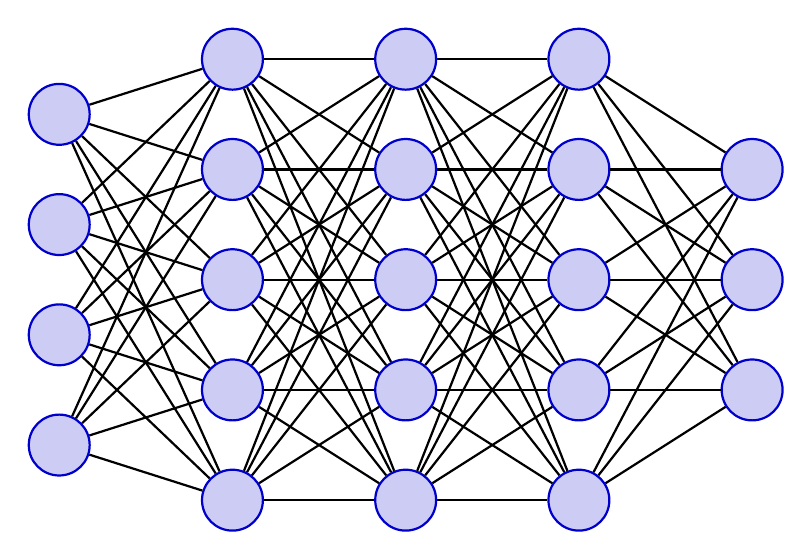
\begin{tikzpicture}[x=2.2cm,y=1.4cm]
  \readlist\Nnod{4,5,5,5,3} % number of nodes per layer
  % \Nnodlen = length of \Nnod (i.e. total number of layers)
  % \Nnod[1] = element (number of nodes) at index 1
  \foreachitem \N \in \Nnod{ % loop over layers
    % \N     = current element in this iteration (i.e. number of nodes for this layer)
    % \Ncnt  = index of current layer in this iteration
    \foreach \i [evaluate={\x=\Ncnt; \y=\N/2-\i+0.5; \prev=int(\Ncnt-1);}] in {1,...,\N}{ % loop over nodes
      \node[mynode] (N\Ncnt-\i) at (\x,\y) {};
      \ifnum\Ncnt>1 % connect to previous layer
        \foreach \j in {1,...,\Nnod[\prev]}{ % loop over nodes in previous layer
          \draw[thick] (N\prev-\j) -- (N\Ncnt-\i); % connect arrows directly
        }
      \fi % else: nothing to connect first layer
    }
  }
\end{tikzpicture}
\end{center}

\end{frame}


\begin{frame}{Linear Model}


\begin{gradblock}{}
    {
    \Huge
    \begin{align*}
    y = wx + b
    \end{align*}
    }
    \end{gradblock}
    
    For $n$ features, and introducing unit feature $x_0 = 1$ to incorporate $b$ into summation as $w_0$
    
    $$
    y = \sum_{i=0}^n w_i x_i
    $$
    
   or
   
   $$
   y = \wbf^\top \xbf
   $$

\end{frame}

\begin{frame}{Perceptron}

\begin{columns}
%------------------------------------------------
\column{.45\textwidth}

A neuron with unit-step for decision making:

\includegraphics[scale=0.55]{figures/Perceptron.pdf}

No hidden layer present.

Unit step is heaviside function \begin{align*}
g(z) = \begin{cases}
1, \quad \text{~~if~~} z \geq \theta\\
0, \quad \text{otherwise}
\end{cases}
\end{align*}

\LARGE

So what could be the problem here?

\column{.45\textwidth}
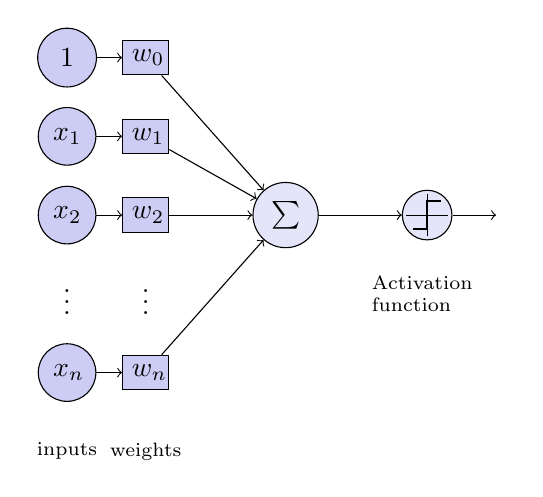
\begin{tikzpicture}
        \node[functions] (center) {};
        \node[below of=center,font=\scriptsize,text width=4em] {Activation function};
        \draw[thick] (0.5em,0.5em) -- (0,0.5em) -- (0,-0.5em) -- (-0.5em,-0.5em);
        \draw (0em,0.75em) -- (0em,-0.75em);
        \draw (0.75em,0em) -- (-0.75em,0em);
        \node[right of=center] (right) {};
            \path[draw,->] (center) -- (right);
        \node[functions,left=3em of center] (left) {$\sum$};
            \path[draw,->] (left) -- (center);
        \node[weights,left=3em of left] (2) {$w_2$} -- (2) node[input,left of=2] (l2) {$x_2$};
            \path[draw,->] (l2) -- (2);
            \path[draw,->] (2) -- (left);
        \node[below of=2] (dots) {$\vdots$} -- (dots) node[left of=dots] (ldots) {$\vdots$};
        \node[weights,below of=dots] (n) {$w_n$} -- (n) node[input,left of=n] (ln) {$x_n$};
            \path[draw,->] (ln) -- (n);
            \path[draw,->] (n) -- (left);
        \node[weights,above of=2] (1) {$w_1$} -- (1) node[input,left of=1] (l1) {$x_1$};
            \path[draw,->] (l1) -- (1);
            \path[draw,->] (1) -- (left);
        \node[weights,above of=1] (0) {$w_0$} -- (0) node[input,left of=0] (l0) {$1$};
            \path[draw,->] (l0) -- (0);
            \path[draw,->] (0) -- (left);
        \node[below of=ln,font=\scriptsize] {inputs};
        \node[below of=n,font=\scriptsize] {weights};
\end{tikzpicture}


\end{columns}



\end{frame}


\begin{frame}{Need for multi-layer perceptron}

\begin{enumerate}
\item A single-layer perceptron is good for linearly separable classes.


\item Optimization does not converge for nonlinearly separable datasets.


\item Non-differentiability of unit-step prevents using gradient descent.

\item A single-layer perceptron lacks generalizability.


\end{enumerate}


\end{frame}


\begin{frame}{Activation function with differentiability}

\begin{enumerate}

\item Sigmoid: \begin{align*}
\sigma(x) = \frac{1}{1 + e^{-x}}
\end{align*}

preferred for predicting probabilities as range is between 0 and 1.

\item Tanh or Hyperbolic tangent:

\begin{align*}
\tanh(x) = \frac{e^x - e^{-x}}{e^x + e^{-x}}
\end{align*}

Suitable for being used as activation functon for hidden layers. Ranges between -1 and +1.

\end{enumerate}

\end{frame}


\begin{frame}{Activation function with differentiability}

\begin{enumerate}

\item Rectified Linear Unit (ReLU): 

\begin{align*}
ReLU(x) = max(0, x)
\end{align*}

Suitable for regression problems. Range between 0 to $\infty$.


\item Leaky ReLU:

\begin{align*}
LeakyReLU(x) = max(0.01*x, x)
\end{align*}

Suitable for regression problems. It solves the problem of dead neuron suffered while ReLU is used, i.e., if a neuron receives only negative inputs, it outputs zero and its gradient becomes zero. This means it stops learning. Leaky ReLU is a modified version of ReLU designed to fix the problem of dead neurons. Instead of returning zero for negative inputs it allows a small, non-zero value.
\end{enumerate}

\end{frame}




\begin{frame}{Activation function with differentiability}

\centering

\includegraphics[scale=0.44]{figures/activation_functions.pdf}

\end{frame}




\section{Training a Simple Neural Network with One Hidden Layer}

\begin{frame}
    \sectionpage
\end{frame}

\begin{frame}{A Simple Neural Network}

\footnotesize

\begin{center}
    
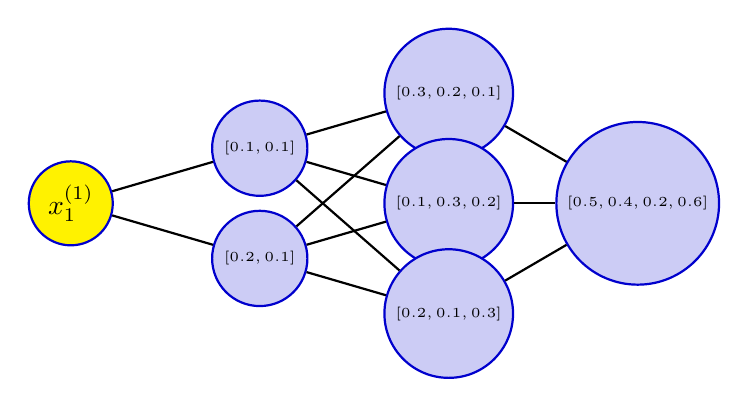
\begin{tikzpicture}[x=2.4cm,y=1.4cm]
  \readlist\Nnod{1, 2, 3, 1} % number of nodes per layer
  
  % Define weights for each layer
  % Layer 1 (input): no weights needed
  \readlist\Wone{{0.1, 0.1}, {0.2, 0.1}, {0.15, 0.2}} % weights for layer 2
  \readlist\Wtwo{{0.3, 0.2, 0.1}, {0.1, 0.3, 0.2}, {0.2, 0.1, 0.3}} % weights for layer 3
  \readlist\Wthree{{0.5, 0.4, 0.2, 0.6}} % weights for output layer

  % \Nnodlen = length of \Nnod (i.e. total number of layers)
  % \Nnod[1] = element (number of nodes) at index 1
  
  \foreachitem \N \in \Nnod{ % loop over layers
    % \N     = current element in this iteration (i.e. number of nodes for this layer)
    % \Ncnt  = index of current layer in this iteration
    \foreach \i [evaluate={\x=\Ncnt; \y=\N/2-\i+0.5; \prev=int(\Ncnt-1);}] in {1,...,\N}{ % loop over nodes
      \ifnum\Ncnt=1 % first layer (input layer)
        \node[mynode, fill=yellow] (N\Ncnt-\i) at (\x,\y) {$x_1^{(1)}$};
      \else\ifnum\Ncnt=2 % hidden layer (second layer)
        \node[mynode] (N\Ncnt-\i) at (\x,\y) {\tiny $[\Wone[\i]]$};
      \else\ifnum\Ncnt=3 % third layer
        \node[mynode] (N\Ncnt-\i) at (\x,\y) {\tiny $[\Wtwo[\i]]$};
      \else % output layer
        \node[mynode] (N\Ncnt-\i) at (\x,\y) {\tiny $[\Wthree[\i]]$};
      \fi\fi\fi
      
      \ifnum\Ncnt>1 % connect to previous layer
        \foreach \j in {1,...,\Nnod[\prev]}{ % loop over nodes in previous layer
          \draw[thick] (N\prev-\j) -- (N\Ncnt-\i); % connect arrows directly
        }
      \fi % else: nothing to connect first layer
    }
  }
\end{tikzpicture}

\end{center}
Each neuron is a denoted by circle consisting of affine part (Linear Model) and activation function.

\begin{enumerate}
\item Single feature, the first layer contains two neurons, one hidden layer with three neurons, and one  output.
\item Consider classification problem either 0 or 1.
\item Superscript $(1)$ means first training sample, subscript $1$ feature index. 
\item Intermediate nodes $\wbf = [w_0, w_1, \ldots]$.
\end{enumerate}

\end{frame}

\begin{frame}{Forward Propagation}
Consider the first training sample $x_1^{(1)} = 2.0$. True label as $1$. Also consider Sigmoid as the activation function, i.e. $\sigma(z) = \frac{1}{1+e^{-z}}$.

Layer 1: 
\begin{enumerate}

\item Neuron 1: $z_1^{[1]} = 0.1 + 0.1\times2.0 = 0.3$. $a_1^{[1]} =  \frac{1}{1+e^{-0.3}}  = 0.5744$.

\item Neuron 2: $z_2^{[1]} = 0.2 + 0.1\times2.0 = 0.4$. $a_2^{[1]} =  \frac{1}{1+e^{-0.4}}  = 0.5987$.

\end{enumerate} 

Here, in an essence, the first layer expands one feature to two features, and basically each neurons will learn something different from the training data.
\end{frame}


\begin{frame}{Forward Propagation}

Layer 2:

\begin{enumerate}
\item Neuron 1: $z_1^{[2]} = 0.3 + 0.2 \times 0.5744 + 0.1 \times 0.5987 =  0.4748$. $a_1^{[2]} = \sigma(0.4748) = 0.6165$.

\item Neuron 2: $z_2^{[2]} = 0.1 + 0.3 \times 0.5744 + 0.2 \times 0.5987 = 0.3921$. $a_2^{[2]} = \sigma( 0.3921) = 0.5968$.

\item Neuron 3: $z_3^{[2]} = 0.2 + 0.1 \times 0.5744 + 0.3 \times 0.5987 =  0.4370$. $a_3^{[2]} = \sigma( 0.4370) = 0.6075$.
\end{enumerate}

\end{frame}

\begin{frame}{Forward Propagation}

Layer 3 (Output):

\begin{enumerate}
\item Output Neuron: $z_1^{[3]} = 0.5 + 0.4 \times 0.6165 + 0.2 \times 0.5968 + 0.6 \times 0.6075 = 1.2305$.
\item $a_1^{[3]} = \sigma(1.2305) =  0.7739$.
\end{enumerate}

The final output $\hat{y} =  0.7739$.
\end{frame}


\begin{frame}{Cross-Entropy Loss Calculation}
Given the true label $y = 1$ and predicted output $\hat{y} = 0.7739$:

\begin{align*}
\text{Cross-Entropy Loss} &= -[y \log(\hat{y}) + (1-y) \log(1-\hat{y})] \\
&= -[1 \cdot \log(0.7739) + 0 \cdot \log(1-0.7739)] \\
&= -\log(0.7739) \\
&= -(-0.2563) \\
&= 0.2563
\end{align*}

Where $\log$ denotes natural logarithm, and $\log(0.7740) \approx -0.2563$.

\vspace{0.5cm}

\begin{itemize}
\item The loss quantifies how well the network's prediction matches the true label.
\item Lower loss indicates better prediction (perfect prediction would give loss = 0).
\item For binary classification with sigmoid activation, cross-entropy loss is commonly used.
\end{itemize}
\end{frame}


\begin{frame}{Cross-Entropy Loss and Its Derivative}
For binary classification with true label $y \in \{0,1\}$ and predicted probability $\hat{y} \in (0,1)$, the cross-entropy loss is:

\begin{align*}
L(y, \hat{y}) &= -[y \log(\hat{y}) + (1-y) \log(1-\hat{y})]
\end{align*}

\textbf{Its derivative:}
\begin{align*}
\frac{\partial L}{\partial \hat{y}} &= \frac{\partial}{\partial \hat{y}}[-y \log(\hat{y}) - (1-y)\log(1-\hat{y})] \\
&= -y \cdot \frac{1}{\hat{y}} \cdot 1 - (1-y) \cdot \frac{1}{1-\hat{y}} \cdot (-1) \\
&= -\frac{y}{\hat{y}} + \frac{1-y}{1-\hat{y}}
\end{align*}

\footnotesize

\begin{itemize}
\item When $y=1$: $\frac{\partial L}{\partial \hat{y}} = -\frac{1}{\hat{y}} + 0 = -\frac{1}{\hat{y}}$
\item When $y=0$: $\frac{\partial L}{\partial \hat{y}} = 0 + \frac{1}{1-\hat{y}} = \frac{1}{1-\hat{y}}$
\item The gradient encourages $\hat{y}$ to move toward $y$ (negative gradient pushes $\hat{y}$ up when $y=1$)
\end{itemize}
\end{frame}

\begin{frame}{Sigmoid Activation Function and Its Derivative}
The sigmoid function and its derivative have a nice property:

\begin{align*}
\sigma(z) &= \frac{1}{1 + e^{-z}} = \hat{y} \\
\frac{d\sigma}{dz} &= \sigma(z)[1 - \sigma(z)] = \hat{y}(1-\hat{y})
\end{align*}

\tiny

\textbf{Derivation:}
\begin{align*}
\frac{d\sigma}{dz} &= \frac{d}{dz}\left(1 + e^{-z}\right)^{-1} \\
&= -(1 + e^{-z})^{-2} \cdot (-e^{-z}) \\
&= \frac{e^{-z}}{(1 + e^{-z})^2} \\
&= \frac{1}{1 + e^{-z}} \cdot \frac{e^{-z}}{1 + e^{-z}} \\
&= \sigma(z) \cdot \left(1 - \frac{1}{1 + e^{-z}}\right) \\
&= \sigma(z)[1 - \sigma(z)]
\end{align*}

 The derivative is expressed in terms of the function value itself . No need to recompute $e^{-z}$.
\end{frame}

\begin{frame}{Chain Rule in Backpropagation}
Backpropagation uses the chain rule from calculus:

If $L = f(g(h(x)))$, then:
\begin{align*}
\frac{\partial L}{\partial x} &= \frac{\partial L}{\partial f} \cdot \frac{\partial f}{\partial g} \cdot \frac{\partial g}{\partial h} \cdot \frac{\partial h}{\partial x}
\end{align*}

\tiny 

\textbf{In Neural Networks:}
\begin{align*}
L &\leftarrow \text{Loss function} \\
\hat{y} &\leftarrow \sigma(z^{[\ell]}) \quad \text{(output activation)}, \ell \text{~denotes layer index} \\
z^{[\ell]} &\leftarrow w^{[\ell]}a^{[\ell-1]} + w_0^{[\ell]} \quad \text{(linear combination)} \\
a^{[\ell-1]} &\leftarrow \sigma(z^{[\ell-1]}) \quad \text{(previous layer activation)}
\end{align*}


\textbf{Gradient flow:}
\begin{align*}
\frac{\partial L}{\partial w^{[\ell]}} &= \frac{\partial L}{\partial \hat{y}} \cdot \frac{\partial \hat{y}}{\partial z^{[\ell]}} \cdot \frac{\partial z^{[\ell]}}{\partial w^{[\ell]}} \\
&= \left(-\frac{y}{\hat{y}} + \frac{1-y}{1-\hat{y}}\right) \cdot \hat{y}(1-\hat{y}) \cdot a^{[\ell-1]}
\end{align*}

\textbf{Note:} $\hat{y}(1-\hat{y})$ cancels when $\hat{y}$ is not 0 or 1, simplifying computation!
\end{frame}

\begin{frame}{These Derivatives Are Well-Behaved}

\footnotesize

\textbf{1. Numerical Stability:}
\begin{itemize}
\item Cross-entropy with sigmoid avoids extreme gradients
\item For $\hat{y} \approx 0$ or $\hat{y} \approx 1$: $\hat{y}(1-\hat{y}) \approx 0$
\item This prevents huge weight updates when confident but wrong
\end{itemize}

\textbf{2. Gradient Behavior:}
\begin{align*}
\frac{\partial L}{\partial z^{[\ell]}} &= \hat{y} - y \quad \text{(after simplification!)}
\end{align*}

\textbf{Derivation:}
\begin{align*}
\frac{\partial L}{\partial z^{[\ell]}} &= \left(-\frac{y}{\hat{y}} + \frac{1-y}{1-\hat{y}}\right) \cdot \hat{y}(1-\hat{y}) \\
&= -y(1-\hat{y}) + (1-y)\hat{y} = -y + y\hat{y} + \hat{y} - y\hat{y} = \hat{y} - y
\end{align*}

\textbf{Beautiful Result:} The gradient is simply the prediction error!
\begin{itemize}
\item When $\hat{y} > y$: Positive gradient decreases weights
\item When $\hat{y} < y$: Negative gradient increases weights
\item Intuitive and numerically stable
\end{itemize}
\end{frame}


\begin{frame}{Backpropagation: Gradient Calculation}
We'll compute gradients using chain rule. Recall: $\hat{y} = 0.7740$, $y = 1$.

\vspace{0.3cm}

\textbf{Step 1: Output Layer Gradient}
\begin{align*}
\frac{\partial L}{\partial \hat{y}} &= -\frac{y}{\hat{y}} + \frac{1-y}{1-\hat{y}} = -\frac{1}{0.7740} + 0 = -1.2922 \\
\frac{\partial \hat{y}}{\partial z^{[3]}} &= \hat{y}(1-\hat{y}) = 0.7739 \times  0.2261 =  0.1750
  \\
\frac{\partial L}{\partial z^{[3]}} &= \frac{\partial L}{\partial \hat{y}} \cdot \frac{\partial \hat{y}}{\partial z^{[3]}} = -1.2922 \times  0.1750 = -0.2261
\end{align*}

\end{frame}


\begin{frame}{Backpropagation: Gradient Calculation}

\textbf{Step 2: Layer 3 Weight Gradients}
\begin{align*}
\frac{\partial z^{[3]}}{\partial w_0^{[3]}} &= 1, \quad
\frac{\partial L}{\partial w_0^{[3]}} = -0.2261 \times 1 = -0.2261 \\
\frac{\partial z^{[3]}}{\partial w_1^{[3]}} &= a_1^{[2]} = 0.6165, \quad
\frac{\partial L}{\partial w_1^{[3]}} = -0.2261 \times 0.6165 = -0.1394 \\
\frac{\partial z^{[3]}}{\partial w_2^{[3]}} &= a_2^{[2]} = 0.5968, \quad
\frac{\partial L}{\partial w_2^{[3]}} = -0.2261 \times 0.5968 = -0.1349 \\
\frac{\partial z^{[3]}}{\partial w_3^{[3]}} &= a_3^{[2]} = 0.6075, \quad
\frac{\partial L}{\partial w_3^{[3]}} = -0.2261 \times 0.6075 = -0.1374
\end{align*}
\end{frame}

\begin{frame}{Backpropagation: Layer 2 Gradients}
\textbf{Step 3: Backpropagate to Layer 2}
\begin{align*}
\frac{\partial L}{\partial a_1^{[2]}} &= \frac{\partial L}{\partial z^{[3]}} \cdot \frac{\partial z^{[3]}}{\partial a_1^{[2]}} = -0.2261 \times 0.4 = -0.0904 \\
\frac{\partial L}{\partial a_2^{[2]}} &= -0.2261 \times 0.2 = -0.0452 \\
\frac{\partial L}{\partial a_3^{[2]}} &= -0.2261 \times 0.6 = -0.1357
\end{align*}

\end{frame}


\begin{frame}{Backpropagation: Gradient Calculation}

\small

\textbf{Step 4: Layer 2 Neuron Gradients}
For each neuron $i$ in layer 2: $\frac{\partial a_i^{[2]}}{\partial z_i^{[2]}} = a_i^{[2]}(1-a_i^{[2]})$
\begin{align*}
\frac{\partial L}{\partial z_1^{[2]}} &= \frac{\partial L}{\partial a_1^{[2]}} \cdot a_1^{[2]}(1-a_1^{[2]}) = -0.0904 \times (0.6165 \times 0.3835) = -0.0904 \times 0.2364 = -0.0214 \\
\frac{\partial L}{\partial z_2^{[2]}} &= -0.0452 \times (0.5968 \times 0.4032) = -0.0452 \times 0.2406 = -0.0109 \\
\frac{\partial L}{\partial z_3^{[2]}} &= -0.1356 \times (0.6075 \times 0.3925) = -0.1356 \times 0.2384 = -0.0323
\end{align*}
\end{frame}

\begin{frame}{Backpropagation: Layer 2 Weight Gradients}

\footnotesize

\textbf{Step 5: Layer 2 Weight Gradients}
For neuron 1 in layer 2:
\begin{align*}
\frac{\partial L}{\partial w_{01}^{[2]}} &= \frac{\partial L}{\partial z_1^{[2]}} \times 1 = -0.0214 \\
\frac{\partial L}{\partial w_{11}^{[2]}} &= \frac{\partial L}{\partial z_1^{[2]}} \times a_1^{[1]} = -0.0214 \times 0.5744 = -0.0123 \\
\frac{\partial L}{\partial w_{21}^{[2]}} &= \frac{\partial L}{\partial z_1^{[2]}} \times a_2^{[1]} = -0.0214 \times 0.5987 = -0.0128
\end{align*}

For neuron 2 in layer 2:
\begin{align*}
\frac{\partial L}{\partial w_{02}^{[2]}} &= -0.0109, \quad
\frac{\partial L}{\partial w_{12}^{[2]}} = -0.0109 \times 0.5744 = -0.0063, \quad
\frac{\partial L}{\partial w_{22}^{[2]}} = -0.0109 \times 0.5987 = -0.0065
\end{align*}

For neuron 3 in layer 2:
\begin{align*}
\frac{\partial L}{\partial w_{03}^{[2]}} &= -0.0323, \quad
\frac{\partial L}{\partial w_{13}^{[2]}} = -0.0323 \times 0.5744 = -0.0186, \quad
\frac{\partial L}{\partial w_{23}^{[2]}} = -0.0323 \times 0.5987 = -0.0193
\end{align*}
\end{frame}

\begin{frame}{Backpropagation: Layer 1 Gradients}

\footnotesize

\textbf{Step 6: Backpropagate to Layer 1}
\begin{align*}
\frac{\partial L}{\partial a_1^{[1]}} &= \sum_{j=1}^3 \frac{\partial L}{\partial z_j^{[2]}} \cdot w_{1j}^{[2]} \\
&= (-0.0214 \times 0.2) + (-0.0109 \times 0.3) + (-0.0323 \times 0.1) \\
&= -0.00428 - 0.00327 - 0.00323 = -0.01078 \\
\frac{\partial L}{\partial a_2^{[1]}} &= (-0.0214 \times 0.1) + (-0.0109 \times 0.2) + (-0.0323 \times 0.3) \\
&= -0.00214 - 0.00218 - 0.00969 = -0.01401
\end{align*}

\textbf{Step 7: Layer 1 Neuron Gradients}
\begin{align*}
\frac{\partial L}{\partial z_1^{[1]}} &= \frac{\partial L}{\partial a_1^{[1]}} \cdot a_1^{[1]}(1-a_1^{[1]}) = -0.01078 \times (0.5744 \times 0.4256) = -0.01078 \times 0.2445 = -0.00264 \\
\frac{\partial L}{\partial z_2^{[1]}} &= -0.01401 \times (0.5987 \times 0.4013) = -0.01401 \times 0.2403 = -0.00337
\end{align*}
\end{frame}

\begin{frame}{Backpropagation: Layer 1 Weight Gradients}

\footnotesize

\textbf{Step 8: Layer 1 Weight Gradients}
For neuron 1 in layer 1 (input $x_1^{(1)} = 2.0$):
\begin{align*}
\frac{\partial L}{\partial w_{01}^{[1]}} &= \frac{\partial L}{\partial z_1^{[1]}} \times 1 = -0.00264 \\
\frac{\partial L}{\partial w_{11}^{[1]}} &= \frac{\partial L}{\partial z_1^{[1]}} \times x_1^{(1)} = -0.00264 \times 2.0 = -0.00528
\end{align*}

For neuron 2 in layer 1:
\begin{align*}
\frac{\partial L}{\partial w_{02}^{[1]}} &= \frac{\partial L}{\partial z_2^{[1]}} \times 1 = -0.00337 \\
\frac{\partial L}{\partial w_{12}^{[1]}} &= \frac{\partial L}{\partial z_2^{[1]}} \times x_1^{(1)} = -0.00337 \times 2.0 = -0.00674
\end{align*}

\vspace{0.3cm}

\textbf{We've computed all gradients needed for weight updates using gradient descent}:
$$\mathbf{w} \leftarrow \mathbf{w} - \eta \frac{\partial L}{\partial \mathbf{w}}$$
where $\eta$ is the learning rate.
\end{frame}

\begin{frame}{Weight Updates with Gradient Descent}

\footnotesize

Using gradient descent with learning rate $\eta = 0.1$ :

$$\mathbf{w}_{\text{new}} = \mathbf{w}_{\text{old}} - \eta \cdot \frac{\partial L}{\partial \mathbf{w}}$$

\textbf{Output Layer Updates:}
\begin{align*}
{w_0}^{[3]}_{\text{new}} &= 0.5 - 0.1 \times (-0.2261) = 0.5 + 0.0226 = 0.5226 \\
{w_1}^{[3]}_{\text{new}} &= 0.4 - 0.1 \times (-0.1393) = 0.4 + 0.01393 = 0.4139 \\
{w_2}^{[3]}_{\text{new}} &= 0.2 - 0.1 \times (-0.1349) = 0.2 + 0.01349 = 0.2135 \\
{w_3}^{[3]}_{\text{new}} &= 0.6 - 0.1 \times (-0.1373) = 0.6 + 0.01373 = 0.6137
\end{align*}
\end{frame}

\begin{frame}{Layer 2 Weight Updates}

\footnotesize


\textbf{Neuron 1 in Layer 2:}
\begin{align*}
w_{01}^{[2]_{\text{new}}} &= 0.3 - 0.1 \times (-0.0214) = 0.3 + 0.00214 = 0.3021 \\
w_{11}^{[2]_{\text{new}}} &= 0.2 - 0.1 \times (-0.0123) = 0.2 + 0.00123 = 0.2012 \\
w_{21}^{[2]_{\text{new}}} &= 0.1 - 0.1 \times (-0.0128) = 0.1 + 0.00128 = 0.1013
\end{align*}

\textbf{Neuron 2 in Layer 2:}
\begin{align*}
w_{02}^{[2]_{\text{new}}} &= 0.1 - 0.1 \times (-0.0109) = 0.1 + 0.00109 = 0.1011 \\
w_{12}^{[2]_{\text{new}}} &= 0.3 - 0.1 \times (-0.0063) = 0.3 + 0.00063 = 0.3006 \\
w_{22}^{[2]_{\text{new}}} &= 0.2 - 0.1 \times (-0.0065) = 0.2 + 0.00065 = 0.2007
\end{align*}

\textbf{Neuron 3 in Layer 2:}
\begin{align*}
w_{03}^{[2]_{\text{new}}} &= 0.2 - 0.1 \times (-0.0323) = 0.2 + 0.00323 = 0.2032 \\
w_{13}^{[2]_{\text{new}}} &= 0.1 - 0.1 \times (-0.0186) = 0.1 + 0.00186 = 0.1019 \\
w_{23}^{[2]_{\text{new}}} &= 0.3 - 0.1 \times (-0.0193) = 0.3 + 0.00193 = 0.3019
\end{align*}
\end{frame}

\begin{frame}{Layer 1 Weight Updates}

\footnotesize


\textbf{Neuron 1 in Layer 1:}
\begin{align*}
w_{01}^{[1]_{\text{new}}} &= 0.1 - 0.1 \times (-0.00264) = 0.1 + 0.000264 = 0.1003 \\
w_{11}^{[1]_{\text{new}}} &= 0.1 - 0.1 \times (-0.00528) = 0.1 + 0.000528 = 0.1005
\end{align*}

\textbf{Neuron 2 in Layer 1:}
\begin{align*}
w_{02}^{[1]_{\text{new}}} &= 0.2 - 0.1 \times (-0.00337) = 0.2 + 0.000337 = 0.2003 \\
w_{12}^{[1]_{\text{new}}} &= 0.1 - 0.1 \times (-0.00674) = 0.1 + 0.000674 = 0.1007
\end{align*}

\vspace{0.5cm}

\begin{itemize}
\item All weights increased slightly because gradients were negative
\item Negative gradient means loss decreases as weight increases
\item Largest updates: Output layer weights (especially bias $w_0^{[3]}$)
\item Smallest updates: First layer weights (vanishing gradient effect)
\item After one training step: Loss should decrease on next forward pass
\end{itemize}
\end{frame}

\begin{frame}{Verification: Forward Pass with New Weights}

\footnotesize


Let's verify the network improves by doing one forward pass with updated weights:

\textbf{Layer 1 with new weights:}
\begin{align*}
z_1^{[1]} &= 0.1003 + 0.1005 \times 2.0 = 0.3013 \quad & a_1^{[1]} &= 0.5748 \\
z_2^{[1]} &= 0.2003 + 0.1007 \times 2.0 = 0.4017 \quad & a_2^{[1]} &= 0.5991
\end{align*}

\textbf{Layer 2 with new weights:}
\begin{align*}
z_1^{[2]} &= 0.3021 + 0.2012 \times 0.5748 + 0.1013 \times 0.5991 = 0.5159 \quad & a_1^{[2]} &= 0.6262 \\
z_2^{[2]} &= 0.1011 + 0.3006 \times 0.5748 + 0.2007 \times 0.5991 = 0.4360 \quad & a_2^{[2]} &= 0.6073 \\
z_3^{[2]} &= 0.2032 + 0.1019 \times 0.5748 + 0.3019 \times 0.5991 = 0.4721 \quad & a_3^{[2]} &= 0.6159
\end{align*}

\textbf{Output Layer with new weights:}
\begin{align*}
z_1^{[3]} &= 0.5226 + 0.4139 \times 0.6262 + 0.2135 \times 0.6073 + 0.6137 \times 0.6159 = 1.3013 \\
\hat{y}_{\text{new}} &= \sigma(1.3013) = 0.7862
\end{align*}
\end{frame}

\begin{frame}{Verification: New Loss Calculation}

\footnotesize


Original prediction: $\hat{y} = 0.7740$, New prediction: $\hat{y}_{\text{new}} = 0.7862$

\textbf{Original Loss:}
$$L = -\log(0.7740) = 0.2563$$

\textbf{New Loss:}
$$L_{\text{new}} = -\log(0.7862) = 0.2404$$

\vspace{0.5cm}

\textbf{Improvement:}
$$\Delta L = 0.2563 - 0.2404 = 0.0159 \quad \text{(6.2\% reduction)}$$

\vspace{0.5cm}

\textbf{Observations:}
\begin{itemize}
\item The network output increased from 0.7740 to 0.7862 (closer to target 1.0)
\item Loss decreased from 0.2563 to 0.2404
\item Gradient descent successfully reduced the loss
\item Multiple epochs (repetitions) would further optimize weights
\end{itemize}

\textbf{Learning Progress:} The network is learning to better predict the true label!
\end{frame}

\begin{frame}{Updated Network Visualization}
\begin{center}
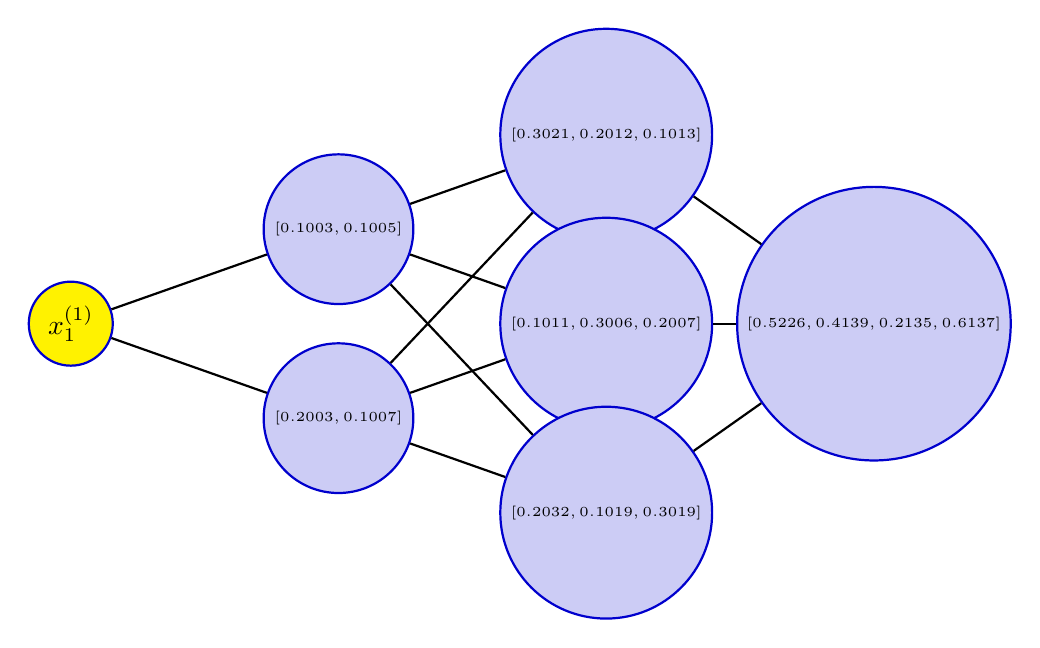
\begin{tikzpicture}[x=3.4cm,y=2.4cm]
  \readlist\Nnod{1, 2, 3, 1}
  
  % Updated weights after one gradient descent step
  \readlist\Wone{{0.1003, 0.1005}, {0.2003, 0.1007}} % Layer 1
  \readlist\Wtwo{{0.3021, 0.2012, 0.1013}, {0.1011, 0.3006, 0.2007}, {0.2032, 0.1019, 0.3019}} % Layer 2
  \readlist\Wthree{{0.5226, 0.4139, 0.2135, 0.6137}} % Output layer
  
  \foreachitem \N \in \Nnod{
    \foreach \i [evaluate={\x=\Ncnt; \y=\N/2-\i+0.5; \prev=int(\Ncnt-1);}] in {1,...,\N}{
      \ifnum\Ncnt=1
        \node[mynode, fill=yellow] (N\Ncnt-\i) at (\x,\y) {$x_1^{(1)}$};
      \else\ifnum\Ncnt=2
        \node[mynode] (N\Ncnt-\i) at (\x,\y) {\tiny $[\Wone[\i]]$};
      \else\ifnum\Ncnt=3
        \node[mynode] (N\Ncnt-\i) at (\x,\y) {\tiny $[\Wtwo[\i]]$};
      \else
        \node[mynode] (N\Ncnt-\i) at (\x,\y) {\tiny $[\Wthree[\i]]$};
      \fi\fi\fi
      
      \ifnum\Ncnt>1
        \foreach \j in {1,...,\Nnod[\prev]}{
          \draw[thick] (N\prev-\j) -- (N\Ncnt-\i);
        }
      \fi
    }
  }
\end{tikzpicture}
\end{center}

\end{frame}

\begin{frame}{At the end of first iteration:}

\begin{itemize}
\item All weights slightly increased (negative gradients)
\item Output layer bias $w_0^{[3]}$ increased most (0.5 → 0.5226)
\item First layer weights changed minimally (vanishing gradient)
\item Network now predicts 0.7862 (improved from 0.7740)
\end{itemize}

\textbf{Next Steps:} Repeat process for entire training dataset over many epochs!
\end{frame}



\section{A Brief Matrix Calculus}

\begin{frame}
    \sectionpage
\end{frame}


\begin{frame}{Derivatives in Neural Network Training}

\begin{enumerate}
\item Training means choose suitable $\wbf$ iteratively.
\item i.e. minimizing a loss function.
\end{enumerate}


Minimize loss $\to$ Gradient Descent $\to$ partial derivative wrt $\wbf$.

\vspace{10pt}

$\wbf$ is a vector.

For neuron, scalar version can work, for multiple neurons, and multiple inputs, it is cumbersome, we need a better frame work, aka Matrix!

\end{frame}



\end{document}